\documentclass[10pt]{article}
\usepackage[top=56pt,bottom=58pt,left=50pt,right=48pt]{geometry}
%\usepackage{apacite}

%\usepackage[
%backend=biber,
%style=nature,
%]{biblatex}

%\usepackage[backend=biber,maxbibnames=2,style=nature,url=false,doi=false,isbn=false,eprint=false,maxcitenames=1,firstinits=false]{biblatex}
%\title{A bibLaTeX example}
%\addbibresource{citations.bib} %Imports bibliography file
%\AtEveryBibitem{\clearfield{pages}} 
%\AtEveryBibitem{\clearfield{number}} 
%\AtEveryBibitem{\clearfield{volume}} 
%\AtEveryBibitem{\clearfield{publisher}} 
%\AtEveryBibitem{\clearfield{month}} 
%\AtEveryBibitem{\clearfield{issue}} 
%\AtEveryBibitem{\clearfield{issn}} 

\usepackage[slovene]{babel}
\usepackage{amsmath}
\usepackage{color}
%\usepackage{graphicx,subfigure}

%\usepackage{subfigure}

\usepackage[T1]{fontenc}
\usepackage[utf8]{inputenc}
\usepackage{lmodern}
\usepackage{amsmath}
\usepackage{tikz}
\usetikzlibrary{shapes,shapes.geometric,arrows,fit,calc,positioning,automata}

\usepackage{amsfonts}
\usepackage{mathrsfs}

\usepackage{float}

\usepackage{caption}
\usepackage{subcaption}

\usepackage{enumerate}

%\usepackage{natbib}

%\usepackage{chemformula}
%\usepackage[version=4]{mhchem}
%\usepackage{mychemistry}
%\usepackage{chemfig}

%\def\phi{\varphi}
%\def\eps{\varepsilon}
%\def\theta{\vartheta}

%\usepackage{physics} ta je za vektorje: \vectorbold{}

%\usepackage{hyperref}
%\hypersetup{
%    colorlinks=true,
%    linkcolor=blue,
%    filecolor=magenta,      
%    urlcolor=cyan,
%    pdftitle={Overleaf Example},
%    pdfpagemode=FullScreen,
%    }
%
%\urlstyle{same}


\newcommand{\thisyear}{2020/21}

\renewcommand{\Re}{\mathop{\rm Re}\nolimits}
\renewcommand{\Im}{\mathop{\rm Im}\nolimits}
\newcommand{\Tr}{\mathop{\rm Tr}\nolimits}
\newcommand{\diag}{\mathop{\rm diag}\nolimits}
\newcommand{\dd}{\,\mathrm{d}}
\newcommand{\ddd}{\mathrm{d}}
\newcommand{\ii}{\mathrm{i}}
\newcommand{\e}{\mathrm{e}}
\newcommand{\lag}{\mathcal{L}\!}
\newcommand{\ham}{\mathcal{H}\!}
\newcommand{\four}[1]{\mathcal{F}\!\left(#1\right)}
\newcommand{\bigO}[1]{\mathcal{O}\!\left(#1\right)}
\newcommand{\sh}{\mathop{\rm sinh}\nolimits}
\newcommand{\ch}{\mathop{\rm cosh}\nolimits}
\renewcommand{\th}{\mathop{\rm tanh}\nolimits}
\newcommand{\erf}{\mathop{\rm erf}\nolimits}
\newcommand{\erfc}{\mathop{\rm erfc}\nolimits}
\newcommand{\sinc}{\mathop{\rm sinc}\nolimits}
\newcommand{\rect}{\mathop{\rm rect}\nolimits}
\newcommand{\ee}[1]{\cdot 10^{#1}}
\newcommand{\inv}[1]{\left(#1\right)^{-1}}
\newcommand{\invf}[1]{\frac{1}{#1}}
\newcommand{\sqr}[1]{\left(#1\right)^2}
\newcommand{\half}{\frac{1}{2}}
\newcommand{\thalf}{\tfrac{1}{2}}
\newcommand{\pd}{\partial}
\newcommand{\Dd}[3][{}]{\frac{\ddd^{#1} #2}{\ddd #3^{#1}}}
%\newcommand{\Pd}[3][{}]{\frac{\pd^{#1} #2}{\pd #3^{#1}}}
\newcommand{\avg}[1]{\left\langle#1\right\rangle}
\newcommand{\norm}[1]{\left\Vert #1 \right\Vert}
\newcommand{\braket}[2]{\left\langle #1 \vert#2 \right\rangle}
%\newcommand{\obraket}[3]{\left\langle #1 \vert #2 \vert #3 \right \rangle}
%\newcommand{\hex}[1]{\texttt{0x#1}}
\newcommand{\vect}[1]{\boldsymbol{#1}}
\renewcommand{\vec}[1]{\overset{\smash{\hbox{\raise -0.42ex\hbox{$\scriptscriptstyle\rightharpoonup$}}}}{#1}}
\newcommand{\bec}[1]{\mathbf{#1}}
\newcommand{\q}[1]{``#1''}
\newcommand{\euler}{\mathrm{e}}


\renewcommand{\iint}{\mathop{\int\mkern-13mu\int}}
\renewcommand{\iiint}{\mathop{\int\mkern-13mu\int\mkern-13mu\int}}
\newcommand{\oiint}{\mathop{{\int\mkern-15mu\int}\mkern-21mu\raisebox{0.3ex}{$\bigcirc$}}}

\newcommand{\wunderbrace}[2]{\vphantom{#1}\smash{\underbrace{#1}_{#2}}}


\newcounter{daggerfootnote}
\newcommand*{\daggerfootnote}[1]{%
    \setcounter{daggerfootnote}{\value{footnote}}%
    \renewcommand*{\thefootnote}{\fnsymbol{footnote}}%
    \footnote[2]{#1}%
    \setcounter{footnote}{\value{daggerfootnote}}%
    \renewcommand*{\thefootnote}{\arabic{footnote}}%
    }

\graphicspath{ {./slike/}{./video/}}



\begin{document}


\begin{titlepage}
\begin{center}
       
       {\sc\Large	Modelska analiza 2}\\
       \vspace*{5cm}
       \Large\textbf{Zaključna naloga - IVP}\\
       \vspace{0.2cm}
       \vspace{1.6cm}
       \largeŽan Butala\\
       \text{vpisna številka: 28222060}
       
       % \vspace{1cm}
       %\begin{figure}[H]
       %	 \centering
       %	\includegraphics[width=10cm]{semafor1.png}
              %\label{fig:graf1}
       %\end{figure}
       \vfill 

       \normalsize

       \vfill

	\normalsize
 
       {\sc 3. avgust 2023\\
	\vspace{0.2cm}
       Univerza v Ljubljani\\
       Fakulteta za matematiko in fiziko\\}
      
\end{center}
\end{titlepage}


\newpage

%\tableofcontents



\section*{Naloga}
Opazuj ravninsko sipanje delca z maso m na potencialu oblike
\begin{equation}
       V (x, y) = x^2y^2 e^{- (x^2 + y^2)}
       \label{eq:potencial}
\end{equation}
ki ima štiri maksimume pri $(x, y) = (1, \pm 1)$ in $(-1, \pm 1)$ z vrednostjo $E_m = 1/\e^2$. Točkast delec z maso $m = 1$ in
energijo $E$ naj vpada proti osrednjemu delu potenciala iz velike oddaljenosti vzporedno z osjo $x$ vzdolž premice, ki je
oddaljena $b$ od osi $x$ (vpadni parameter).
\begin{figure}[H]
       \hspace*{-0.1cm}
       \centering
       \includegraphics[height=7cm]{potencial1.png}
       \caption{Oblika potenciala.}
       \label{fig:potencial}
\end{figure}










\section{Uvod}
Obravnavamo delec z maso $m$, ki se siplje na analitičnem potencialu $V(x,y)$.
Gibanje je ravninsko, torej bo naš sistem opisan dvema koordinatama in dvema komponentama gibalne količine.
Dinamiko takega sistema lahko kompaktno zapišemo z enačbama
\begin{equation}
       \begin{split}
              \dot {\bec{q}} &= \frac{\partial H}{\partial \bec{p}}, \\
              \dot {\bec{p}} &= -\frac{\partial H}{\partial \bec{q}},
       \end{split}
       \label{eq:hamilton}
\end{equation}
kjer je $H(\bec{q}, \bec{p}) = \frac{\bec{p}^2}{2m} + V(\bec{q})$, potencial pa je podan v navodilu (\ref*{eq:potencial})
To rešujemo kot $\dot{\textbf{y}}= \textbf{f}(y, t)$; $\textbf{y}=(\textbf{q},\textbf{p})^T$, kar poznamo pod imenom začetni problem (IVP).
Enačba \ref{eq:hamilton} je diferencialna enačba drugega reda, kar prepišemo na sistem enačb prvega reda.
Po komponentah se izraža kot:
\begin{equation}
       \begin{split}
              \dot x = & u, \\
              \dot y = & v, \\
              \dot u = & 2xy^2 \, \e^{-(x^2+y^2)} \bigl( -1 + x^2 \bigr), \\
              \dot v = & 2x^2y \, \e^{-(x^2+y^2)} \bigl( -1 + y^2 \bigr).
       \end{split}
       \label{eq:sistem1}
\end{equation}
To rešujemo z integracijskimi algoritmi, ki smo jih spoznali in obdelali na začetku semestra, zato bom ponovno analizo in primerjavo metod v tej nalogi izpustil.
Če na kratko povzamem, smo pri prvi nalogi primerjali metode z adaptivnim korakom in simplektične integratorje ter ugotovili,
 da se pri kaotičnih sistemih oziroma v okolici divje spreminjajočih potencialov najbolje obnese \texttt{odeint}.
Za referenco si lahko ogledamo sliko \ref{fig:odeint}, ki prikazuje gibanje točkastega delca v Coluombskem potencialu.
\begin{figure}[H]
       \hspace*{-0.1cm}
       \centering
       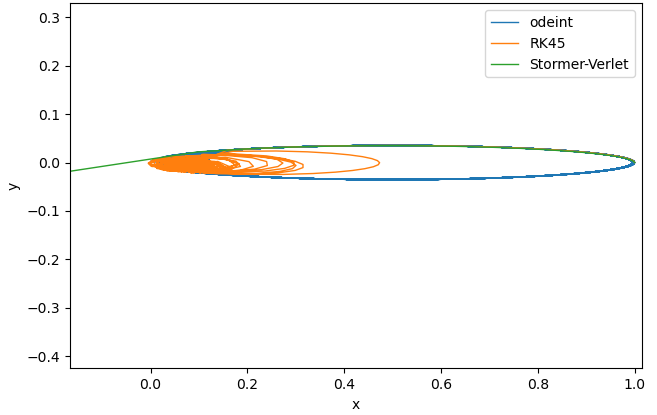
\includegraphics[height=5.5cm]{1orbite7.png}
       \caption{Delovanje numeričnih integratorjev v divje spreminjajočem potencialu.}
       \label{fig:odeint}
\end{figure}









\section{Osnovni rezultati}


\begin{figure}[H]
       \hspace*{-0.1cm}
       \centering
       \begin{subfigure}[b]{0.48\textwidth}
              \centering
              \includegraphics[width=0.9\textwidth]{zgled1.png}
              \caption{ }
       \end{subfigure}
       \begin{subfigure}[b]{0.48\textwidth}
              \centering
              \includegraphics[width=0.9\textwidth]{zgled2.png}
              \caption{ }
       \end{subfigure}
       \caption{(a) Trajektorije delcev z različnim odmikom od simetrale in (b) trajektoriji dveh delcev z istim začetnim pogojem, vendar zasukanim potencialom.}
       \label{fig:zgleda}
\end{figure}
Naloga narekuje spreminjanje parametra odmika $b$ prečno na smer hitrosti, temu pa sem dodal še kot zamika potenciala (slika \ref{fig:zgleda}).
Zanimiva količina za opazovanje je kot končne hitrosti glede na vpadno v odvisnosti od odmika $b$.
V okolici vrhov dobimo divje fluktuacije (slika \ref{fig:fraktali}), ki imajo, kot bomo videli, nekaj zanimivih lastnosti. 

\begin{figure}[H]
       \hspace*{-0.1cm}
       \centering
       \begin{subfigure}[b]{0.48\textwidth}
              \centering
              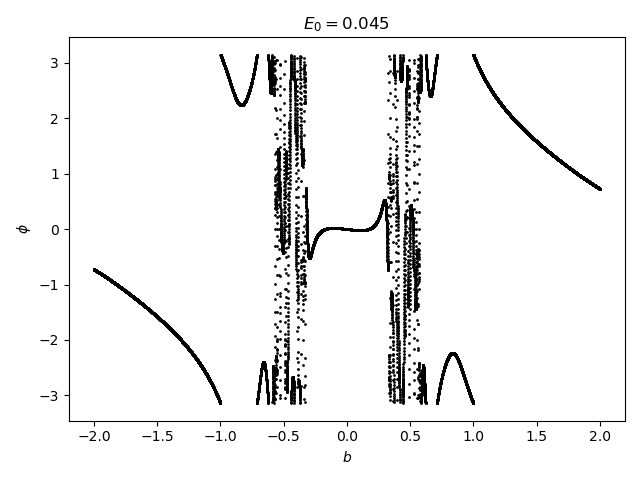
\includegraphics[width=\textwidth]{kot1.png}
              \caption{ }
       \end{subfigure}
       \begin{subfigure}[b]{0.48\textwidth}
              \centering
              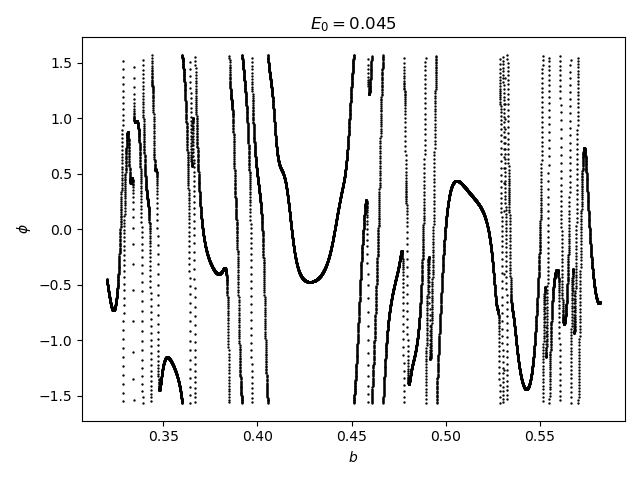
\includegraphics[width=\textwidth]{kot3.png}
              \caption{ }
       \end{subfigure}
       \caption{(a) Odvisnost končnega kota delca glede na vpadnico in (b) povečava na manjši interval.}
       \label{fig:fraktali}
\end{figure}








\section{Kaos}
\subsection{Lyapunov eksponent}
\begin{figure}[H]
       \centering
       \begin{subfigure}[t]{0.40\textwidth}
              \hspace*{-7mm}
              \vspace*{-7mm}
              \centering
              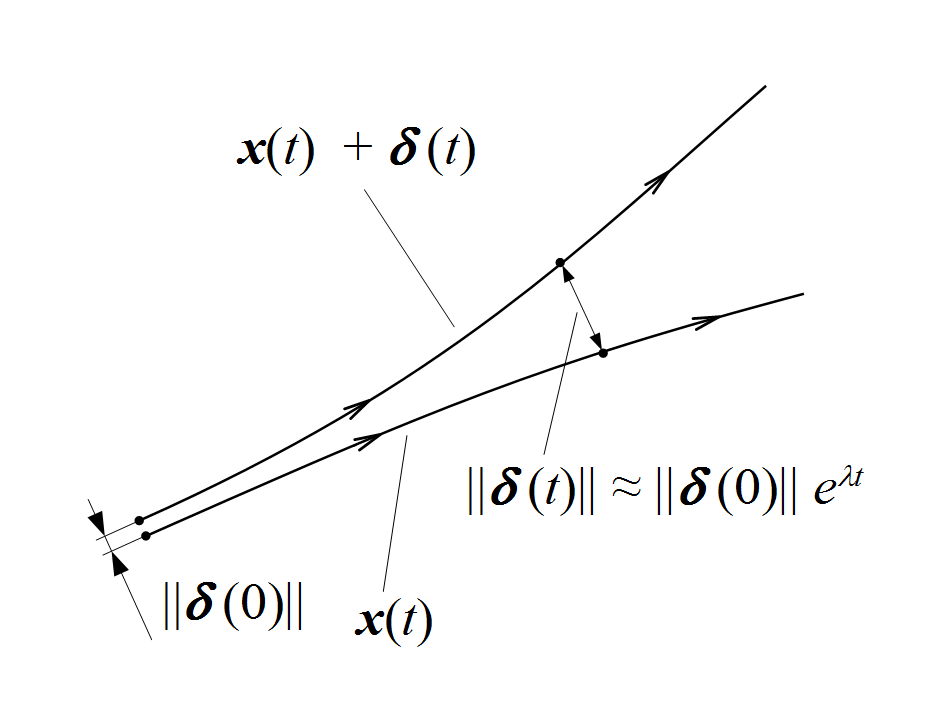
\includegraphics[width=0.8\textwidth]{ljapunov1.png}
              %\caption{}
              \label{fig:kaos0a}
       \end{subfigure}
       \begin{subfigure}[t]{0.40\textwidth}
              \hspace*{0mm}
              \centering
              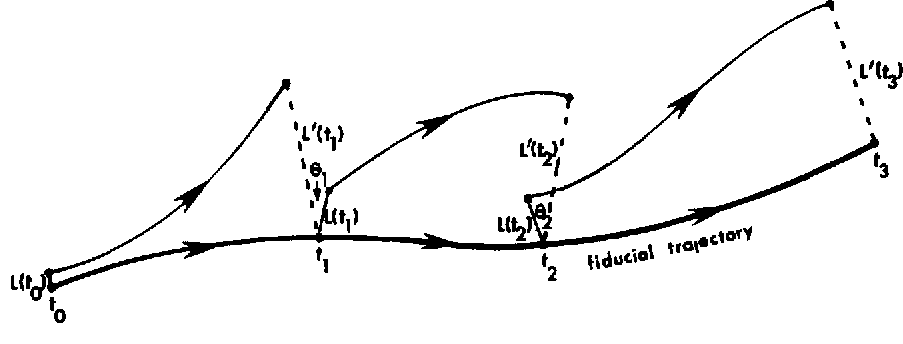
\includegraphics[width=1\textwidth]{ljapunov0.png}
              %\caption{}
              \label{fig:kaos0b}
       \end{subfigure}
       \caption{Ideja Lyapunovega algoritma \cite{shuster}.}
       \label{fig:kaos0}
\end{figure}
Najenostavnejša mera za kaos je Lyapunov exponent $\lambda$ in opisuje občutljivost sistema na začetne pogoje.
Osnovna ideja je, da se v kaotičnih sistemih dve bližnji trajektoriji oddaljujeta exponentno hitro, 
exponent, ki parametrizira to oddaljevanje pa se imenuje Lyapunov exponent.
Definiran je kot
\begin{equation}
       \lambda(x_0) = \lim_{t \rightarrow \infty} \lim_{\delta \rightarrow 0} \frac{\ln \delta(t) / \delta_0}{t},
\end{equation}
kjer je $\delta (t)$ razdalja med dvema točkama tekom časovne evolucije, $\delta_0$ pa je razdalja med njima na začetku.
Drugo limito lahko priredimo za potrebe numeričnega izračuna in sicer tako, da gledamo razdalje vsakih $k$ korakov, nato pa napravimo reskalacijo nazaj na razdaljo $\varepsilon \equiv \delta_0$ (slika \ref*{fig:kaos0}).
Matematično je to ekvivalentno kot, če bi dve trajektoriji na začetku zbližali za produkt vseh reskalacij (izognemo se omejitvi float natančnosti).
Lyapunov exponent se nato prevede na
\begin{equation}
       \lambda(x_0) = \lim_{t \rightarrow \infty} \frac{1}{t} \sum_i \ln \frac{\delta(t_i)}{\varepsilon}.
       \label{eq:ljap2}
\end{equation}
kjer so $t_i$ časi reskalacij.
Rezultat prikazuje slika \ref{fig:ljapunov}, kjer vidimo, da so vse limite enake nič.
To je posledica dejstva, da imamo opravka z sipalnim potencialom, ki je pri velikih razdaljah eksponentno zastrt.
Posledično je oddaljevanje dveh bližnih trajektorij pri časih $t \gg 1$ kvečjemu linearno.
Iz slike je razviden logaritemski padec pred interakcijo, nato sledi zanimiv del, kjer se Ljapunov eksponent akumulira in na koncu limitacija proti nič.
Pri tipičnih kaotičnih sistemih, na primer sklopljeni nihali, dobimo prav tako začetni logaritemski padec, nato pa se vzpostavi ravnovesje med prispevki reskalacij in $1/t$ odvisnostjo
v enačbi (\ref{eq:ljap2}), in dobimo vodoravno asimptotiko.
\begin{figure}[H]
       \hspace*{-0.1cm}
       \centering
       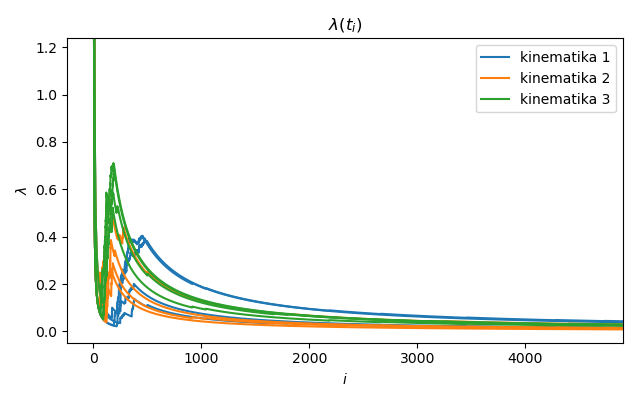
\includegraphics[height=7cm]{ljapunov_final.png}
       \caption{Limitiranje Ljapunovega eksponenta.}
       \label{fig:ljapunov}
\end{figure}




\subsection{Hausdorffova fraktalna dimenzija}

Najprej me je zanimalo, ali lahko vzorčim parameter $b$ tako gosto, da bo zares razvidna krivulja.
To pomeni, da od izbrane točke nobena ni oddaljena manj kot predhodnja in naslednja po parametru $b$.
\begin{figure}[H]
       \centering
       \begin{subfigure}[t]{0.48\textwidth}
              \centering
              \includegraphics[width=1\textwidth]{locljivost3.png}
              \caption{}
              \label{fig:locljivost1a}
       \end{subfigure}
       \begin{subfigure}[t]{0.48\textwidth}
              \hspace*{0mm}
              \centering
              \includegraphics[width=1\textwidth]{visje1.png}
              \caption{}
              \label{fig:locljivost1b}
       \end{subfigure}
       \caption{(a) Število fraktalnih točk v odvisnosti od gostote vzorčenja parametra $b$ in (b) pripadajoče odvisnosti končnega kota od začetnega zamika.}
       \label{fig:locljivost1}
\end{figure}
Pričakovali bi, da bosta za dovolj majhen $\Delta b$ tudi dve zaporednji točki prišli blizu skupaj (delte in epsiloni večji od nič).
Slika \ref{fig:locljivost1a} pa prikazuje, ravno nasprotno.
Na ordinatni osi je narisano število točk, ki imajo vsaj eno nesosednjo točko bližje, kot sosednjo.
Recipročna odvisnost od prikazuje, da se z gostejšim vzorčenjem parametra $b$ rojevajo nove divje oscilacije znotraj kaotičnih intervalov.
To namiguje na fraktalno strukturo.
Pri vse višji energiji vpadnega delca potencial vedno manj vpliva na končno smer.
Sipanj pri velikih kotih je vse manj in krivulja $\theta (b)$ se začne izravnavati.
S tem fraktalna struktura izgine zato je tudi število takih točk takrat enako nič.

Formalno se opisa tega pojava lotimo s Hausdorffovo dimenzijo, ki je mera \q{fraktalnosti}.
V polnem prostoru definiramo celice dimenzije $\varepsilon$ in z njimi pokrivamo fraktalno podmnožico.
Hausdorffova dimenzija je nato definirana kot:
\begin{equation}
       d_H = - \lim_{\varepsilon \rightarrow 0} \frac{\ln N}{\ln \varepsilon},
\end{equation}
kjer je $N$ število celic, ki jih potrebujemo, da prekrijemo celotno fraktalno podmnožico.
Za polne množice je $d_H$ celo število, in je 1 za enodimenzonalno krivuljo v prostoru, 2 za ploskev in tako naprej.

%Algoritem hitro preverimo na znanem zgledu, ki je analitično rešljiv, na primer Sierpinski predpražnik (carpet).
%Zanj velja $d_H = \ln 8/ \ln 3 \approx 1.89$.

\begin{figure}[H]
       \centering
       \begin{subfigure}[t]{0.45\textwidth}
              \centering
              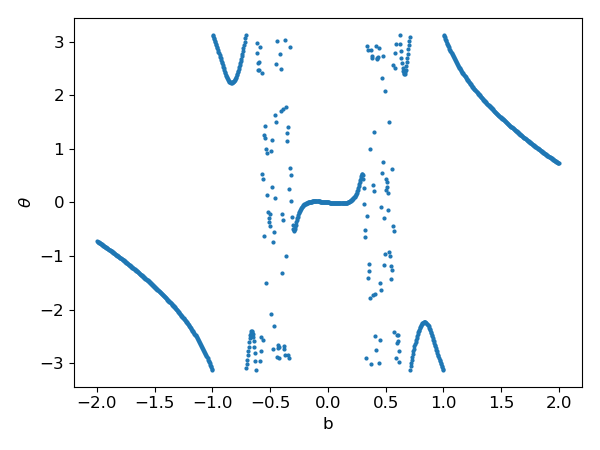
\includegraphics[width=1\textwidth]{hausdorff1_887a.png}
              \caption{}
              \label{fig:hausdorff0a}
       \end{subfigure}
       \begin{subfigure}[t]{0.45\textwidth}
              \hspace*{0mm}
              \centering
              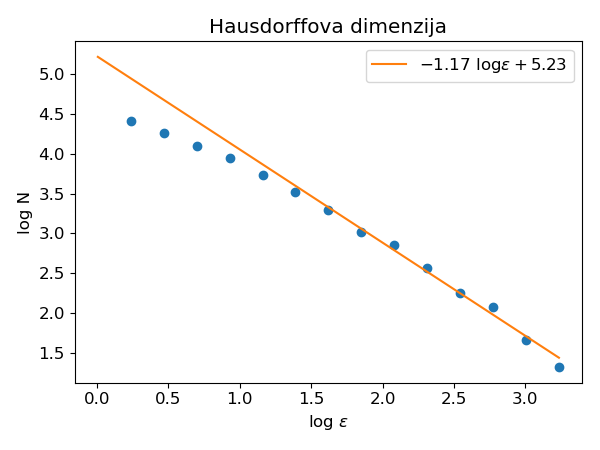
\includegraphics[width=1\textwidth]{hausdorff1_100.png}
              \caption{}
              \label{fig:hausdorff0c}
       \end{subfigure}
       \caption{(a) Odvisnost končnega kota delca od začetnega zamika $b$ in (b) Hausdorffova fraktalna dimenzija.}
       \label{fig:hausdorff0}
\end{figure}


%Preverimo delovanje algoritma z znanimi primeri, ki jim lahko Hausdorffovo dimenzijo določimo analitično.
%%Countable sets have Hausdorff dimension 0.[8]
%%The Euclidean space 
%%R
%%n
%%{\displaystyle \mathbb {R} ^{n}} has Hausdorff dimension 
%%n
%%{\displaystyle n}, and the circle 
%%S
%%1
%%{\displaystyle S^{1}} has Hausdorff dimension 1.[8]
%%Fractals often are spaces whose Hausdorff dimension strictly exceeds the topological dimension.[5] For example, the Cantor set, a zero-dimensional topological space, is a union of two copies of itself, each copy shrunk by a factor 1/3; hence, it can be shown that its Hausdorff dimension is ln(2)/ln(3) ≈ 0.63.[9] The Sierpinski triangle is a union of three copies of itself, each copy shrunk by a factor of 1/2; this yields a Hausdorff dimension of ln(3)/ln(2) ≈ 1.58.[1] These Hausdorff dimensions are related to the "critical exponent" of the Master theorem for solving recurrence relations in the analysis of algorithms.
%
%\begin{figure}[H]
%       \centering
%       \vspace*{-0mm}
%       \begin{subfigure}[t]{0.44\textwidth}
%              \centering
%              %\hspace*{+0mm}
%              \includegraphics[width=1\textwidth]{sierp_2187.png}
%              \caption{}
%              \label{fig:hausdorff1a}
%       \end{subfigure}
%       \vspace*{+0mm}
%       \begin{subfigure}[t]{0.48\textwidth}
%              %\vspace*{+2mm}
%              \centering
%              %\vspace*{+0mm}
%              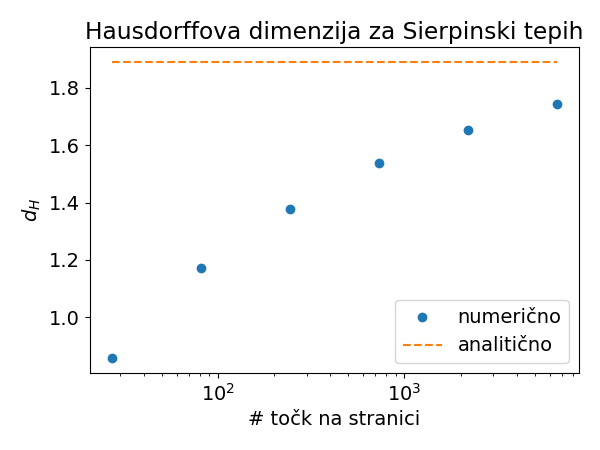
\includegraphics[width=1\textwidth]{hausdorff_sierp_analit.png}
%              \caption{}
%              \label{fig:hausdorff1b}
%       \end{subfigure}
%       \caption{(a) Sierpinski \q{tepih} in (b) primerjava numeričnega izračuna fraktalne dimenzije z analitično.}
%       \label{fig:hausdorff1}
%\end{figure}
V našem primeru bi pričakovali, da bo torej enaka 1, saj je končno stanje pri dani energiji delca določeno s parametrom $b$.
Slika \ref{fig:hausdorff0} pa kaže nekoliko več, torej je množica fraktalna.
Poglejmo si podrobneje.

%Fraktalna dimenzija mora litmitirati proti pravi vrednosti, bližje ko smo analitični množici.
V našem primeru vidimo na sliki \ref{fig:nas} očiten razcep fraktalne dimenzije za razllične kinematike.
Izkaže se, da pri dovolj veliki energiji potencial le malo zmoti delec in zastre fraktalni del, kot je razvidno iz slike \ref{fig:locljivost1b}.
\begin{figure}[H]
       \centering
       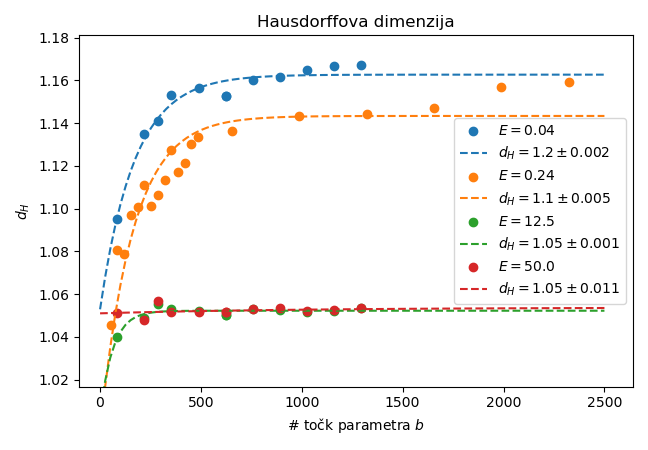
\includegraphics[width=0.5\textwidth]{hausdorff_final.png}
       \caption{Asimptotika Hausdorffove dimenzije pri različnih kinematikah.}
       \label{fig:nas}
\end{figure}












\section{Premik in rotacija polja}
Enako kot za sipan delec lahko po 3. Newtnovem zakonu sestavimo tudi enačbe za premik polja.
Označimo koordinati težišča polja s $(c,s)$.
Sistem enačb za traslacijo je potem:
\begin{equation}
       \begin{split}
              \dot{c} = &\, č, \\
              \dot{s} = &\, š, \\
              \dot{č} = &\, \frac{1}{M} 2xy^2 \, \euler^{-(x^2+y^2)} \, \bigl( 1 - x^2 \bigr), \\
              \dot{š} = &\, \frac{1}{M} 2x^2y \, \euler^{-(x^2+y^2)} \, \bigl( 1 - y^2 \bigr).
       \end{split}
       \label{eq:sistem2}
\end{equation}
Potencial nato na vsakem koraku transformiramo $V(x,y) \rightarrow V(x-c,y-s)$.

Ker je polje razsežno lahko enako napravimo tudi za zasuk.
Newtnow zakon za vrtenje se glasi:
\begin{equation}
       \bec{M} = J \dot{\bec{\omega}},
       \label{eq:newt_vrtenje}
\end{equation}
kjer je $J$ vztrajnostni moment polja.
Ker smo v 2D ravnini, lahko vektorske znake spuščamo in se osredotočimo le na $z$ komponento.
V enačbi (\ref{eq:newt_vrtenje}) upoštevamo $\bec{M} = \bec{r} \times \bec{F}$,  $\bec{F} = -\nabla V$ in dobimo:
\begin{equation}
       \bec{\dot{\omega}} = \frac{ (\bec{r} \times \bec{F})_z }{J_z} = - \frac{ (\bec{r} \times \nabla V(\bec{r}))_z }{J_z}.
\end{equation}
Predpostavimo, da je masna gostota polja $\rho$ sorazmerna s potecialom $V$, ki ima maso $M$ (konceptualno se nič ne spremeni, če $J$ obravnavamo kot neodvisen parameter).
Komponenta vztrajnostnega tenorja $J_z$ se tedaj izraža kot:
\begin{equation}
       J_z = M \iint  V(x,y)\, (x^2+y^2) \dd x \dd y = \frac{3}{4} \pi M.
\end{equation}
Izračun gradienta potenciala in vektorskega produkta nas privede do sistema enačb za zasuk potenciala $V$ okoli osi $z$ za kot $\varphi$:
\begin{equation}
       \begin{split}
              \dot{\varphi} =& \omega, \\
              \dot{\omega} =& - \frac{2x^3y \, \euler^{-x^2-y^2} \, \bigl(-1+y^2\bigr) - 2xy^3 \, \euler^{-x^2-y^2} \, \bigl(-1+x^2\bigr)}{\frac{3}{4}\pi M}.
       \end{split}
       \label{eq:sistem3}
\end{equation}
Ideja je, da enačbe (\ref{eq:sistem1}), (\ref{eq:sistem2}) in (\ref{eq:sistem3}) združimo v en sklopljen sistem enačb.
Rešitve so zelo intuitivne zato sem napravil tudi video animacije, ki so na voljo na \\
\texttt{https://drive.google.com/drive/folders/1jTHFnaiJAKIV3\_Zvb7obxIUQCOwar2pT?usp=sharing}
  oziroma na \\
 \texttt{https://www.youtube.com/playlist?list=PLtan1s3tU6GyEILj5FuTSBOaJChZ7KZSL}.
%\href{https://drive.google.com/drive/folders/1jTHFnaiJAKIV3_Zvb7obxIUQCOwar2pT?usp=sharing}{https://drive.google.com/drive/folders/1jTHFnaiJAKIV3}
%in \href{https://www.youtube.com/playlist?list=PLtan1s3tU6GyEILj5FuTSBOaJChZ7KZSL}{https://www.youtube.com/playlist}.
Za kompletnost poročila so izseki prikazani na slikah \ref{fig:odriv1}, \ref{fig:odriv2} in \ref{fig:odriv3}.

\begin{figure}[H]
       \centering
       \begin{subfigure}[t]{0.32\textwidth}
              \centering
              \includegraphics[width=1\textwidth]{premik1_1040.png}
              %\caption{}
              \label{fig:o1a}
       \end{subfigure}
       \begin{subfigure}[t]{0.32\textwidth}
              \centering
              \includegraphics[width=1\textwidth]{premik1_1060.png}
              %\caption{}
              \label{fig:1b}
       \end{subfigure}
       \begin{subfigure}[t]{0.32\textwidth}
              \centering
              \includegraphics[width=1\textwidth]{premik1_1080.png}
              %\caption{}
              \label{fig:1b}
       \end{subfigure}
       \begin{subfigure}[t]{0.32\textwidth}
              \centering
              \includegraphics[width=1\textwidth]{premik1_1100.png}
              %\caption{}
              \label{fig:o1a}
       \end{subfigure}
       \begin{subfigure}[t]{0.32\textwidth}
              \centering
              \includegraphics[width=1\textwidth]{premik1_1120.png}
              %\caption{}
              \label{fig:1b}
       \end{subfigure}
       \begin{subfigure}[t]{0.32\textwidth}
              \centering
              \includegraphics[width=1\textwidth]{premik1_1140.png}
              %\caption{}
              \label{fig:1b}
       \end{subfigure}

       \caption{Izseki animacije sipanja delca na masivnem potencialu, kjer upoštevamo samo translacijski del interakcije.}
       \label{fig:odriv1}
\end{figure}


\begin{figure}[H]
       \centering
       \begin{subfigure}[t]{0.32\textwidth}
              \centering
              \includegraphics[width=1\textwidth]{zasuk1_1040.png}
              %\caption{}
              \label{fig:o1a}
       \end{subfigure}
       \begin{subfigure}[t]{0.32\textwidth}
              \centering
              \includegraphics[width=1\textwidth]{zasuk1_1060.png}
              %\caption{}
              \label{fig:1b}
       \end{subfigure}
       \begin{subfigure}[t]{0.32\textwidth}
              \centering
              \includegraphics[width=1\textwidth]{zasuk1_1080.png}
              %\caption{}
              \label{fig:1b}
       \end{subfigure}
       \begin{subfigure}[t]{0.32\textwidth}
              \centering
              \includegraphics[width=1\textwidth]{zasuk1_1100.png}
              %\caption{}
              \label{fig:o1a}
       \end{subfigure}
       \begin{subfigure}[t]{0.32\textwidth}
              \centering
              \includegraphics[width=1\textwidth]{zasuk1_1120.png}
              %\caption{}
              \label{fig:1b}
       \end{subfigure}
       \begin{subfigure}[t]{0.32\textwidth}
              \centering
              \includegraphics[width=1\textwidth]{zasuk1_1140.png}
              %\caption{}
              \label{fig:1b}
       \end{subfigure}

       \caption{Izseki animacije sipanja delca na masivnem potencialu, kjer upoštevamo samo rotacijski del interakcije.}
       \label{fig:odriv2}
\end{figure}

\begin{figure}[H]
       \centering
       \begin{subfigure}[t]{0.32\textwidth}
              \centering
              \includegraphics[width=1\textwidth]{oboje2_1040.png}
              %\caption{}
              \label{fig:o1a}
       \end{subfigure}
       \begin{subfigure}[t]{0.32\textwidth}
              \centering
              \includegraphics[width=1\textwidth]{oboje2_1060.png}
              %\caption{}
              \label{fig:1b}
       \end{subfigure}
       \begin{subfigure}[t]{0.32\textwidth}
              \centering
              \includegraphics[width=1\textwidth]{oboje2_1080.png}
              %\caption{}
              \label{fig:1b}
       \end{subfigure}
       \begin{subfigure}[t]{0.32\textwidth}
              \centering
              \includegraphics[width=1\textwidth]{oboje2_1100.png}
              %\caption{}
              \label{fig:o1a}
       \end{subfigure}
       \begin{subfigure}[t]{0.32\textwidth}
              \centering
              \includegraphics[width=1\textwidth]{oboje2_1120.png}
              %\caption{}
              \label{fig:1b}
       \end{subfigure}
       \begin{subfigure}[t]{0.32\textwidth}
              \centering
              \includegraphics[width=1\textwidth]{oboje2_1140.png}
              %\caption{}
              \label{fig:1b}
       \end{subfigure}

       \caption{Izseki animacije sipanja delca na masivnem potencialu z vztrajnostnim momentom $J = 3/4 \pi M$.}
       \label{fig:odriv3}
\end{figure}











\section{Zaključek}
V nalogi smo si ogledali sipanje delca na netrivialnem potencialu.
Sistem je močno občutljiv na spremembo začetnih pogojev, kar smo videli  
Teorija kaosa stereotipno velja za kompleksno in matematično rigurozno področje, vendar se je tekom reševanja ta naloga iz numeričnega stališča vseeno izkazala za morda nekoliko lažjo od ostalih.
Zaradi sipalne narave problema propadejo tudi pristopi, kot so Lyapunov spekter, Poincarejeve sečne ploskve in N-torusi v faznem prostoru, s katerimi sicer analiziramo kaotične sisteme z omejenim faznim prostorom.
Trke dveh in treh točkastih teles s Coluombskimi potenciali smo obdelali v nalogi z dvozvezdjem, zato se mi je ta naloga zdela odlična priložnost za obravnavo sipanja razsežnega telesa in dodatkom enačb gibanja.





%\begin{thebibliography}{widest entry}
%       \bibitem{ss} Širca, S. \& Horvat, M. \emph{Računske metode za fizike} (DMFA - založništvo, 2010),
%\end{thebibliography}

\begin{thebibliography}{9}
       \bibitem{ss} 
       Širca, S. \& Horvat, M. 
       \emph{Računske metode za fizike} (DMFA - založništvo, 2010),
       
       \bibitem{shuster}
       Heinz Georg Schuster, Wolfram Just, \emph{Deterministic Chaos: An Introduction}
       
       \bibitem{prosen}
       Prosen T., Horvat M.
       \emph{Teorija dinamičnih sistemov}, nedokončana skripta.
\end{thebibliography}


\end{document}